\section{Strumentazione}
	Per effettuare tale misurazioni abbiamo impiegato 
	\begin{itemize}[$\cdot$]
		\item Un multimetro digitale
		\item Un righello risoluzione 1 \si{mm}
		\item Un metro a nastro risoluzione 1 \si{cm}
		\item Due bobine di Helmotz, di raggio $r=$\SI{15}{cm} e 130 spire, impiegate per generare il campo magnetico
		\item Un bulbo, fornito di tubo catodico, usato qale cannone elettronico per la 
			generazione degli \e.
			Il bulbo risulta riempito con un gas di elio rarefatto 
			per ottenere una traccia visiva del moto degli \e.
			
		\item Alimentatori per regolare le tensioni e le correnti impiegate.
		\item Una scala gradata, retro illuminata quale riferimento per il moto
		\item Una macchina fotografica digitare, per effettuare le acqusizioni degli
			\e
	\end{itemize}	
\section{Procedimento}	
	\subsection{calibrazione strumentale e verifica delle approssimazioni}	
		Prima di effettare le acqusizioni vere e proprie l'apparato impiegato necessita di una 
		fase di regolazione.
		
		Essendo l'aparato sensibile al campo magnetico terrestre
		con una bussola si è individuata l'orientazione di $B_{terrestre}$
		e si sono orientate le bobine in modo da minizzare l'inflenza.
		L' orientazione delle bobine impiegata pone il campo $B_{terrestre}$ e $B_z$
		prodotto dalle bobine, ortogonali;In tale caso l'influenza
		di $B_{terrestre}$ sul moto degli elettroni porterebbe una variazione
		in profondità; pertanto ininfluente sulla successiva analisi dati,
		che effettua una proiezione sul piano X-Y.
		
		Essendo inoltre la sonda ad effetto Hall sensibile in lettura ai
		campi magnetici residui,  si è andati a modificare gli off-sett del circuito di amplificazione della stessa sonda.
		Per fare tale calibrazione dello zero strumentale si agisce sl potenziometro del circito sino 
		a quando ruotando di \ang{180} la sonda,la lettura non sia 
		uguale in modulo e opposte in segno.
		
		Effettuato ciò si sono alimentate le bobine con una tensione $V_{coil}=$\SI{7.5 \pm 0.1}{\volt}\footnote{Tali misure sono state prese dalla lettura del dispositivo di lettura.
		Si è assunto come errore un digit; a cui eventualmente andrebbero
		aggiunti errori sistemetici dovuti alla calibrazione dell'apparato
		di lettura.}
		attenendo una corrente $I_{coil}=$\SI{0.95 \pm 0.01}{\ampere}\footnote[1]{}
		;
		dopodichè si è mappato il campo $B_z$ sul
		piano di moto degli \e, in funzione della distanza dal centro per un intorno \SI{\pm 6}{cm} del centro della spira $centro_{spira}=20$cm. si è ritenuta tale regione come area di interesse poiché si essendo il raggio del bulbo approssimativamente di $5-6$ cm, il moto gli elettroni osservabili si svolge entro tale intervallo.
		Per effettare tale osservazioni si è impiegata la sonda ad effetto Hall.	
		La sonda restituisce un segnale in tensione ,che amplificato da un circuito,
		di guadagno noto $G=11.1 \pm 0.1$ $$controllare$$, viene letta attraverso il multimetro 
		in dotazione.Si è associata alla lettura un incertezza di 1 digit.
		La posizione della sonda è stata calcolata impiegando il righello in dotazione.
		
		Si riportano i valori ottenuti da tale mappatura in 
		\begin{table}[hb]
			\centering
			\begin{tabular}{|c|c|c|}
				\toprule
				$r $\SI{\pm 0.1}{cm} & 	$V_{out}$ \SI{\pm 0.001}{ \volt} \\
				\midrule
				14.0 		& 	\SI{ 0.405 \pm 0.001}{\volt} \\
				14.5		& 	\SI{ 0.407 \pm 0.001}{\volt} \\
				15.0		& 	\SI{ 0.408 \pm 0.001}{\volt} \\
				15.5		& 	\SI{ 0.408 \pm 0.001}{\volt} \\
				16.0		& 	\SI{ 0.408 \pm 0.001}{\volt} \\
				16.5		& 	\SI{ 0.409 \pm 0.001}{\volt} \\
				17.0		& 	\SI{ 0.409 \pm 0.001}{\volt} \\
				17.5		& 	\SI{ 0.409 \pm 0.001}{\volt} \\
				18.0		& 	\SI{ 0.409 \pm 0.001}{\volt} \\
				18.5		& 	\SI{ 0.409 \pm 0.001}{\volt} \\
				19.0		& 	\SI{ 0.409 \pm 0.001}{\volt} \\
				19.5		& 	\SI{ 0.409 \pm 0.001}{\volt} \\
				20.0		& 	\SI{ 0.409 \pm 0.001}{\volt} \\
				20.5		& 	\SI{ 0.410 \pm 0.001}{\volt} \\
				21.0		& 	\SI{ 0.410 \pm 0.001}{\volt} \\
				21.5		& 	\SI{ 0.409 \pm 0.001}{\volt} \\
				22.0		& 	\SI{ 0.410 \pm 0.001}{\volt} \\
				22.5		& 	\SI{ 0.410 \pm 0.001}{\volt} \\
				23.0		& 	\SI{ 0.410 \pm 0.001}{\volt} \\
				23.5		& 	\SI{ 0.409 \pm 0.001}{\volt} \\
				24.0		& 	\SI{ 0.409 \pm 0.001}{\volt} \\
				24.5		& 	\SI{ 0.409 \pm 0.001}{\volt} \\
				25.0		& 	\SI{ 0.408 \pm 0.001}{\volt} \\
				25.5		& 	\SI{ 0.407 \pm 0.001}{\volt} \\
				26.0		& 	\SI{ 0.406 \pm 0.001}{\volt} \\
				
				\bottomrule
			\end{tabular}
			\caption{Si riporta la lettura della sonda ad effetto Hall in funzione
				della posizione della posizione della stessa.
				Per effettare una misura comoda delle posizioni si è effettuata una
				misura dall'esterno ottenedo $r_{centro}=20$ cm}
				%Si ricorda 
			%	Dal principio di sovrapposizione e il campo di una bobina sul campo otteniamo un campo atteso
		%$B_{atteso}=\mu_0\frac{R^2}{{(R^2+z^2)}^{3/2}}I_{coil}=$}
			\label{t:a}
		\end{table}	
	\tab{a}
	Dai dati tabulati si è effettuato un grafico di $V_{out,z}/V_{out}^{max}$;
	avendo stabilito una corrispondenza biunivaca $B$ ed $V$ misurato;
	si è assunto la sostanziale corrispondenza tra il grafico di $V_{out,z}/V_{out}^{max}$ ed un grafico di $B_{out,z}/B_{out}^{max}$.
	\begin{figure}[hb]
		\centering
		\subfloat[fit di  $V_{out,z}/V_{out}^{max}$]{
			\includegraphics[scale=0.5]{./fig/figure_1.png}
			\label{f:1}
		}\\
		\subfloat[andamento previsto]{
			\includegraphics[scale=0.5]{./fig/andamento.pdf}
			\label{f:andamento} 
		}
		\caption{grafico corrispondente ad un grafico di $B_{out,z}/B_{out}^{max}$ VS $r$}
		\label{fig:fit1}
	\end{figure}
	
	
	
	Si riporta l'andamento fittato in \figurename{ \ref{f:1}}.
	
	Da un confronto tra l'andamento trovato e qello previsto
	si è osservato un sostanziale accordo.
	si osserva inoltre che per una regione compresa tra $r_{min}=15$ e $r_{max}=25$ 
	il campo magnetico $B_z$ può essere considerato uniforme; pertanto in linea con 
	le esigenze sperimentali.
	Dalle specifiche della sonda allo stato solido si ottiene $B_{z,max}= $\SI{7.37	\pm 1.6	}{\milli \tesla}
	$$errore da rivedere$$ ed	$B_{z,atteso}= $\SI{7.41	\pm 0.08	}{\milli \tesla} si ottiene anche un sostanziale accordo tra il valore massimo verificato e quello previsto.
	
	Per la trattazione di eventali aberrazioni dovte alla lente della fotocamera
	si effettata una foto della scala gradata posta dietro la seconda bobina sia a bulbo disinserito che a seguito della sua inserzione.
	\begin{figure}[hb]
		\centering
		\subfloat[assenza bulbo]{
			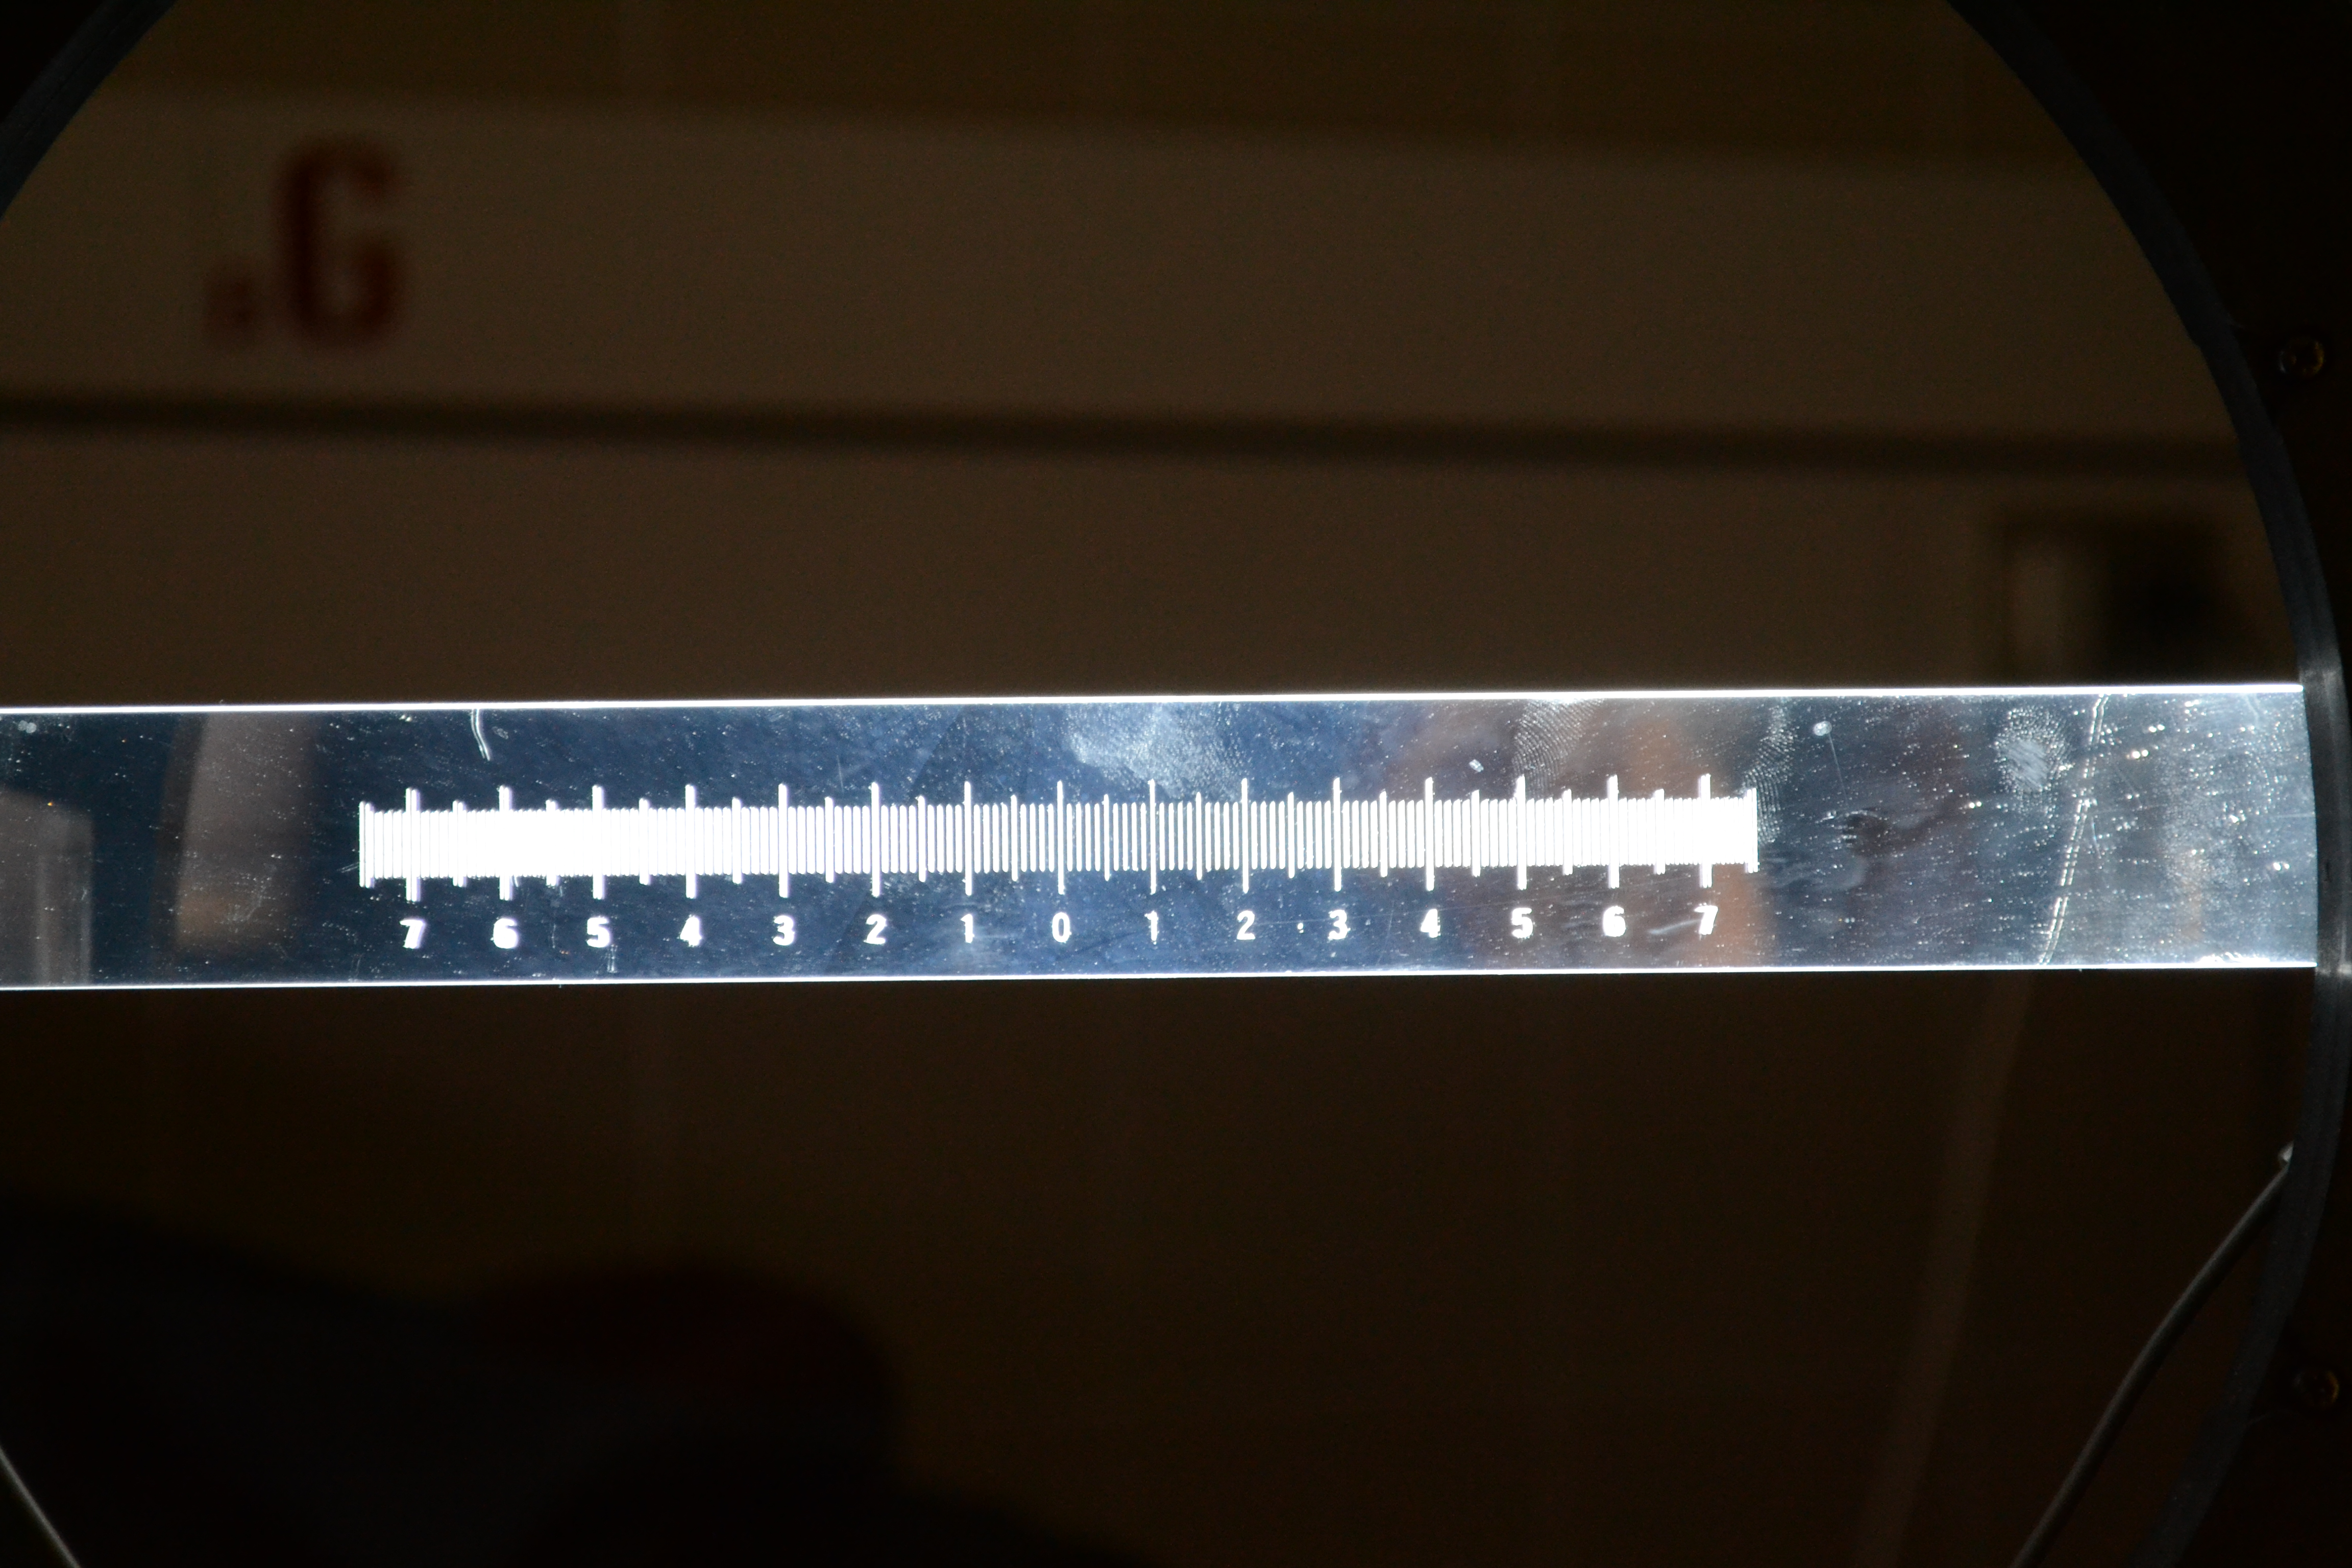
\includegraphics[scale=0.35]{./fig/NO.JPG}
			\label{f:scalano}
		}\\
		\subfloat[bulbo inserito]{
			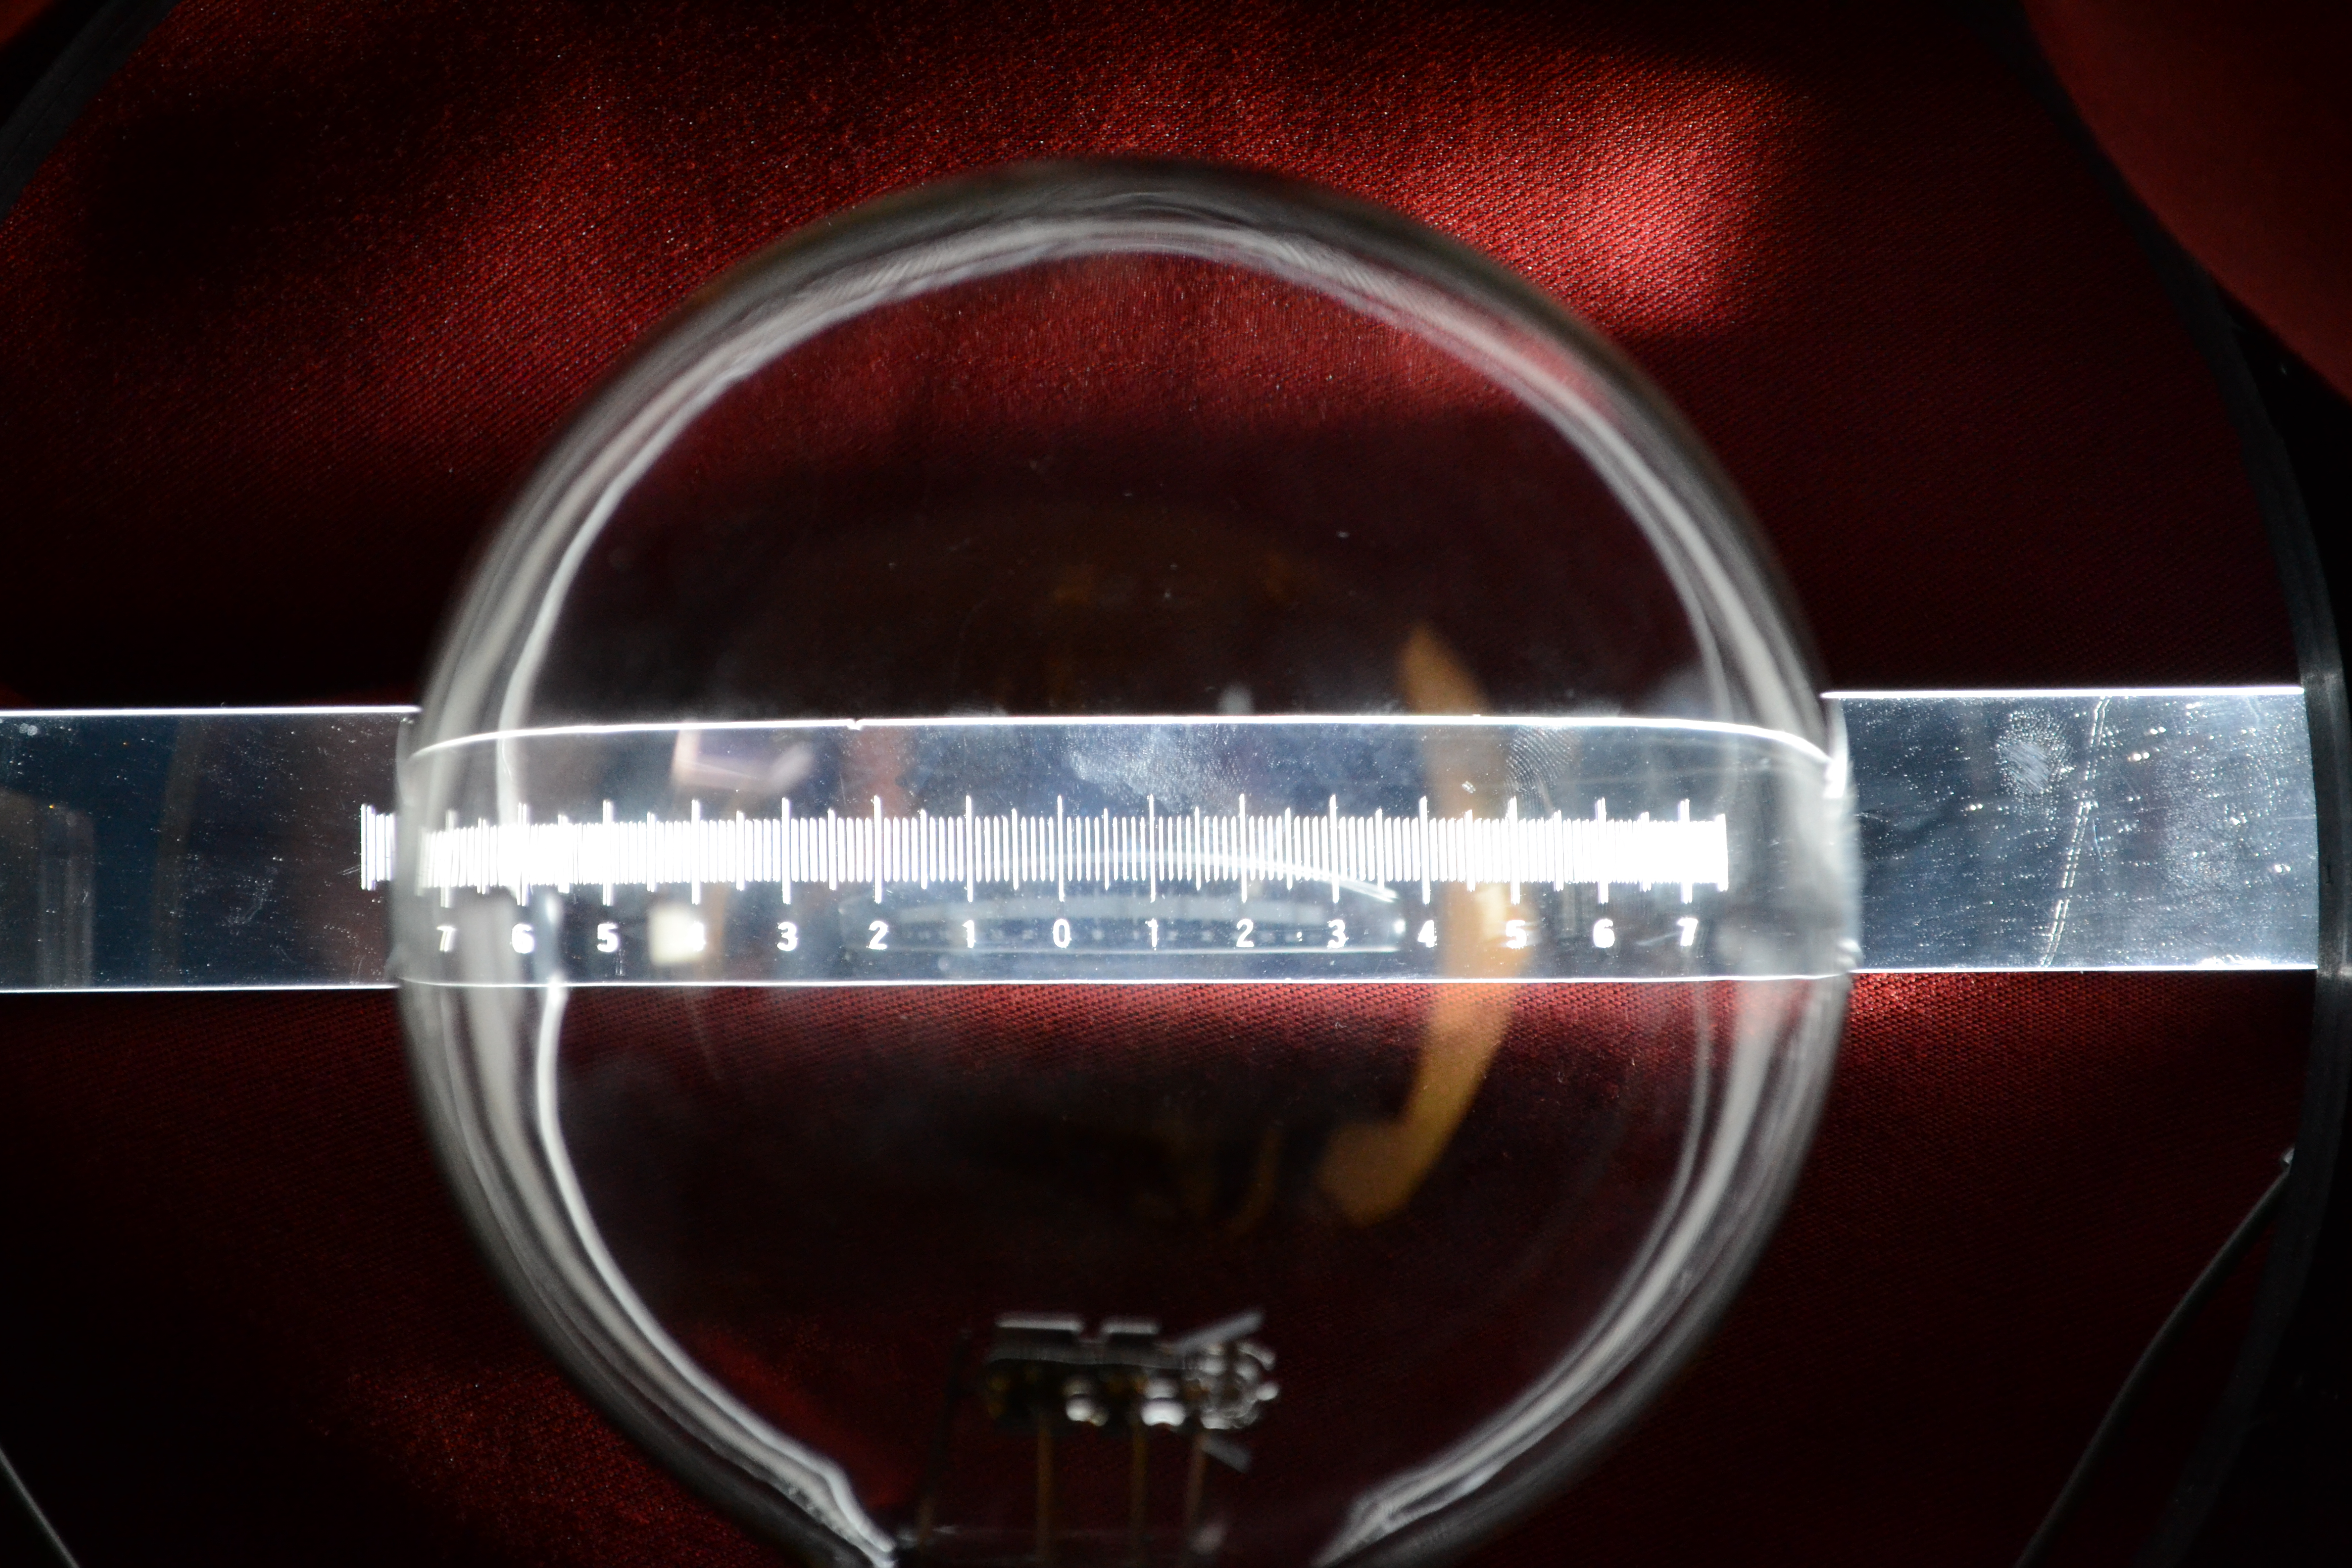
\includegraphics[scale=0.35]{./fig/SI.JPG}
			\label{f:scalasi} 
		}
		\caption{foto della scala gradata posta dietro la seconda bobina sia a bulbo disinserito che a seguito della sua inserzione.}
		\label{f:scala}
	\end{figure}
	
	
	
	
	
	
	
	
	
	
	
	
	
	
	
	
	
	
	
	
	
	